\section{The gate model and quantum circuits}

This section briefly reviews the gate model for circuit based quantum computing and discusses the similarities between between digital and quantum computers. The gate model is one of the most popular architectures for quantum computation at the moment. A number of companies such as, \textit{Intel \cite{intelqcomp} IBM \cite{ibmqweb}, Google \cite{googleqai} and Rigetti \cite{rigetti}} are all using the gate model approach for quantum computing. There are other architectures for quantum computing however we think that the gate model is the most similar to digital computers.

Both forms of computation follow the same structure, you start with bits (or qubits), operations are performed on the (qu)bits and then you measure the new values of the (qu)bits. We show an example in \autoref{fig:basicoperation}.

%%%% digital circuit
\begin{figure}[H] 
\centering
\begin{subfigure}[h]{0.4\textwidth}
\begin{align*}
\Qcircuit @C=0.5cm @R=0.7cm
{&\lstick{A} &\multigate{2}{Operation} & \\
&\lstick{B} &\ghost{Operation} & \\
&& &\qw &\lstick{Q} \\}
\end{align*}
\caption{Digital operation}
\label{fig:digitalcirc}
\end{subfigure}
~
%%%% Q circuit
\begin{subfigure}[H]{0.4\textwidth}
\begin{align*}
\Qcircuit @C=0.5cm @R=0.7cm
{&\lstick{A} &\multigate{2}{Operation} &\qw &\lstick{A} \\
&\lstick{B} &\ghost{Operation} &\qw &\lstick{B} \\
&\lstick{Q} &\ghost{Operation} &\qw &\lstick{Q} \\}
\end{align*}
\caption{Quantum operation}
\label{fig:quantumcirc}
\end{subfigure}
\caption{Digital and quantum logic circuits for implementing an arbitrary operation on bits $A, B$ returning value $Q$}
\label{fig:basicoperation}
\end{figure}

One of the main differences between the two figures is that in the quantum circuit the inputs $A \& B$ exist after the operation and the output $Q$ is present before the operation. This is a feature of quantum computing being reversible (unitary).  

One of the requirements for quantum computing to be universal is that we are able to perform any single qubit and a single two qubit gate. Most quantum algorithms make use of a Hadamard gate at the beginning of the computation. 


\begin{figure}[H]
    \begin{align*}
    \Qcircuit @C=0.5cm @R=0.7cm
    {&\lstick{0} &\gate{H} &\qw &\rstick{\frac{0+1}{\sqrt{2}}} \\ 
    &\lstick{A} &\qw &\qw &\rstick{A} }
    \end{align*}
    \caption{Hadamard gate acting on the top qubit and no gate performed on the bottom qubit}
    \label{fig:my_label}
\end{figure}


Multiple qubits gates are of the form, control-\textit{Operation}, one of the most popular two-qubit gates used is the Controlled-NOT. The control means use the value of the first qubit to decide whether or not to perform the operation on the target qubit. 


\begin{figure}[H]
    \begin{align*}
    \Qcircuit @C=0.5cm @R=0.7cm
    {&\lstick{0} &\gate{H} &\qw &\rstick{0 \text{  if  } A=0, \frac{0+1}{\sqrt{2}} \text{  if  } A=1 } \\ 
    &\lstick{A} &\ctrl{-1} &\qw &\rstick{A} }
    \end{align*}
    \caption{Hadamard gate acting on the top qubit and no gate performed on the bottom qubit}
    \label{fig:my_label}
\end{figure}



\subsubsection{Digital logic}

Every digital computing operation can be built up from NAND logic gates \cite{sheffer1913set}. We can call a NAND logic gate a universal gate for computation. The NOR gate is also universal in the same way any computation can be constructed from NOR gates.

\begin{figure}[H]
  \centering
  \begin{subfigure}[h]{0.4\textwidth}
  \centering
  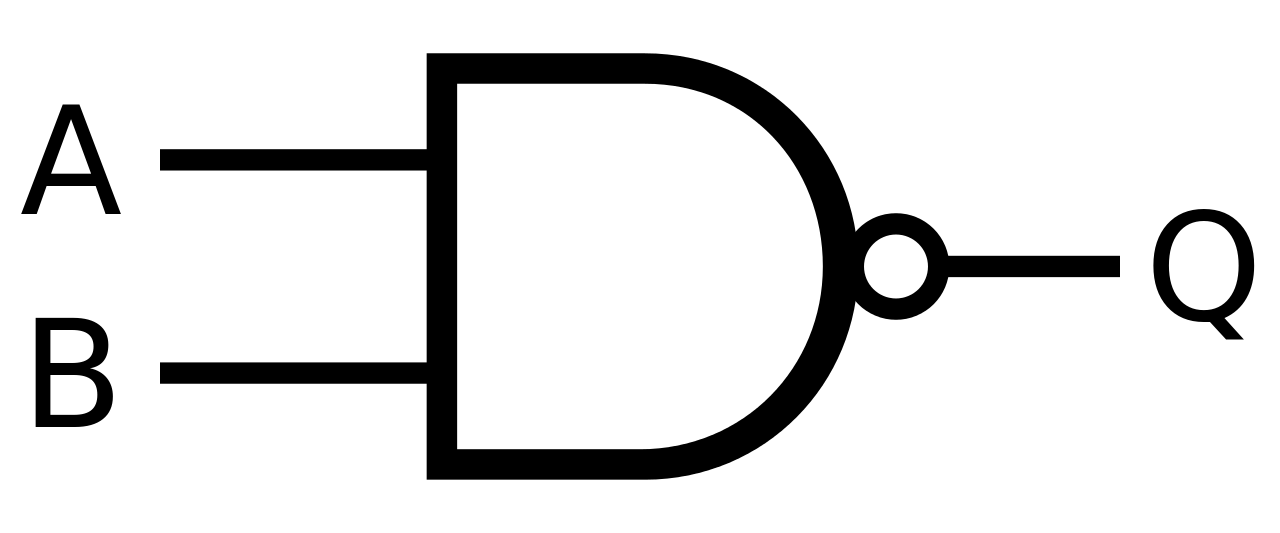
\includegraphics[width=0.7\textwidth]{NAND_ANSI_Labelled_svg.png}
  \caption{The NAND logic gate \cite{nandwiki}.}
  \label{fig:NAND}
\end{subfigure}
~
  \begin{subfigure}[h]{0.4\textwidth}
  \centering
  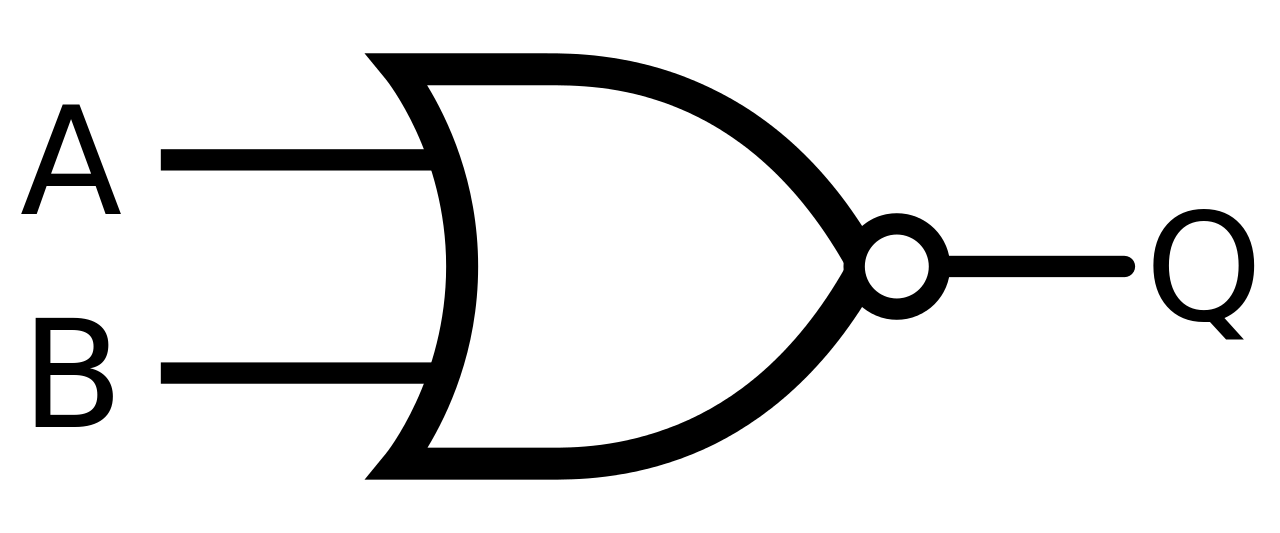
\includegraphics[width=0.7\textwidth]{NOR_ANSI_Labelled_svg.png}
  \caption{The NOR logic gate \cite{norwiki}.}
  \label{fig:NOR}
  \end{subfigure}
\end{figure}

\begin{table}[!htb]
    \caption{Global caption}
    \begin{subtable}{.5\linewidth}
      \centering
        \begin{tabular}{|l|l||l|}
        \hline
        Input A & Input B & Output Q \\ \hline
        0       & 0       & 1       \\ 
        0       & 1       & 0       \\ 
        1       & 0       & 0       \\ 
        1       & 1       & 0       \\
        \hline
    \end{tabular}
    \caption{NOR gate truth table}
    \end{subtable}
    %
    \begin{subtable}{.5\linewidth}
      \centering
        \begin{tabular}{|l|l||l|}
        \hline
        Input A & Input B & Output Q \\ \hline
        0       & 0       & 1       \\ 
        0       & 1       & 1       \\ 
        1       & 0       & 1       \\ 
        1       & 1       & 0       \\
        \hline
    \end{tabular}
    \caption{NAND gate truth table}
    \end{subtable} 
\end{table}


\begin{comment}
reversible logic




%%%%%%%%% circuit 1 
\begin{figure}[h!]
\begin{align*}
\Qcircuit @C=0.5cm @R=0.7cm
{%1
&\lstick{S_1} &\gate{H} &\ctrl{1} &\qw \\
%0
&\lstick{S_0} &\ctrl{-1} &\targ &\qw \\}
\end{align*}
\caption{Schur transform for 2 qubits}
\label{cir:vanilla2}
\end{figure}

\end{comment}